\section{Introductory Example} 

We now present a simple example to give an overview of our Verilog to C translation and to illustrate how properties for safety verification written in System Verilog Assertions (SVA) will be translated into C code for our experiments. We assume the reader is familiar with the basics of Verilog and SVA~\cite{verilog}. \tmcmt{Rajdeep - please add the best references for Verilog and SVA.}

Fig.\ \ref{fig:example} shows a typical Verilog module with a variety of common constructs: register datatypes, initialization, non-blocking and blocking assignments, an assign statement, and procedural blocks.  The synthesized hardware is the simple circuit shown in the centre.  On the right is the result of our translation of this Verilog RTL code into C.

The details of the translation are explained in Sec.\ \ref{sec:v2c}. In summary, all the state-holding registers in the Verilog design have been gathered into a C struct. A function \texttt{top} is then defined that has the same parameters as the Verilog module it represents. When invoked, this function executes a sequence of state updates that simulate a single clock-cycle of hardware execution, according to the Verilog synthesis semantics. Because this is a sequentialization of the parallel register updates modelled by the Verilog, some shadow variables are introduced that record register values at the start of the clock cycle for subsequent use.  The non-synthesizable Verilog {\bf\texttt{initial}} block is not included here; it is a testbench component, and not part of the circuit.  Placement of the assignment to \texttt{c} at the end of the body of \texttt{top} follows the `read after write' semantics for Verilog combinational logic.

In our experiments, we compare safety verification of SVA properties of Verilog RTL and software analysis tools of the corresponding C code.  
We translate SVA into equivalent C code. A collection of typical SVA properties is shown below:

\begin{center}
\begin{tabular}[t]{@{}l@{}}
\begin{lstlisting}[mathescape=true,language=Verilog,basicstyle=\scriptsize\ttfamily]
P0: assert property (d >= e);
P1: assert property ((a == 1) |-> ##1 (b == 1));
P2: assert property ((a == 1) |-> ##2 (e == 1));
P3: assert property ((a == 1) |-> ##3 (d == 2));
P4: assert property ((a == 0) |-> ##4 (out == 1));
P5: assert property ((a == 1) |-> ##4 (out == 4));
\end{lstlisting}
\end{tabular}
\end{center}

\noindent These are conditional properties, each spanning a fixed number of clock cycles. 
 
The corresponding C is shown in Fig.\ \ref{fig:sva}. After a block of assignments that do the initialization, we have a non-terminating while-loop that models a continuously-running system. In each iteration of the loop, we invoke the \texttt{top} function of the software netlist for simulating advancement of the hardware clock by one cycle.   We model the varying input signal \texttt{a} by assigning a fresh, `non-deterministic' value at the start of each iteration. The history of values on this input is recorded in an array \texttt{hist}; we set a bound of 100 for the while loop, and so this array need hold the values of the input signal at only the first 100 clock cycles. 

An SVA property is valid (true) if it holds at the end of every clock cycle. In the C code, the corresponding assertion must also hold at every iteration of the loop. An SVA implication of the form \texttt{(P |-> \#\#N Q)}, where \texttt{P} is a condition on input \texttt{a}, therefore gets translated into a C assertion that \texttt{Q} holds whenever the relevant past values of \texttt{a} satisfy \texttt{P}. We discuss property translation in more detail in Sec.\ \ref{sec:props}.

\begin{figure}[t]
\small
\begin{center}
\begin{tabular}{l}
\hline\noalign{\vskip0.25ex}
\textbf{Property Checking Testbench in C} \\
\hline
\begin{lstlisting}[boxpos=t,mathescape=true,language=C,basicstyle=\scriptsize\ttfamily]
int main() 
{
 _Bool hist[100];
 _Bool clk, a;
 unsigned char c, out;
 unsigned int cycle=1;
 // initial block for top module
 u1.b=0;u1.d=0; u1.e=0;u1.out=0; 
 
 while(cycle <= 100) {
   // read non-deterministic value of 'a'
   a = nondet_bool(); 
   // record value of 'a' in current cycle
   hist[cycle] = a;
   // invoke top-level function
   top(clk,a,&c,&out);
   // increment cycle count
   cycle=cycle+1; 
   // assert global properties 
   P0:assert(u1.d>=u1.e);
   // properties with antecedent a==1 
   // property with 1 cycle delay
   if (cycle>1 && hist[cycle-1]==1) 
     P1:assert(u1.b==1);
   // property with 2 cycle delay
   if (cycle>2 && hist[cycle-2]==1)
      P2:assert(u1.e==1); 
   // property with 3 cycle delay
   if (cycle>3 && hist[cycle-3]==1)
      P3:assert(u1.d==2); 
   // property with 4 cycle delay
   if (cycle>4 && hist[cycle-4]==1)
      P5:assert(u1.out==4); 
   // properties with antecedent a==0
   // property with 4 cycle delay
   if (cycle>4 && hist[cycle-4]==0) 
     P4:assert(u1.out==1);
 }
}
\end{lstlisting}\\
\hline
\end{tabular}
\caption{Translation of SVA Properties into C}
\label{fig:sva}
\end{center}
\end{figure}

The waveform in Fig.\ \ref{intro-waveform} shows the input-output behavior of the RTL design. 
Using state-of-the-art verifiers, we prove that the result of all the SVA properties 
are the same in the RTL and the software netlist. For example, the properties \texttt{P2} and \texttt{P3} 
hold only for the first cycle in both RTL and software netlist; they fail in the 
subsequent cycles in both models.  All other properties 
hold globally in both models.
%
\begin{figure} 
\begin{center}
  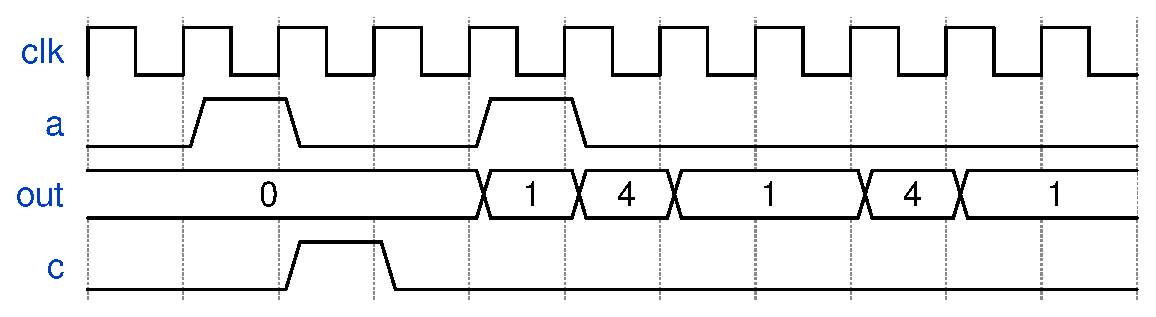
\includegraphics[width=\columnwidth]{figures/example/waveform1.eps}%
	\caption{Waveform Showing the Input-Output Behaviour of the RTL in Fig.~\ref{fig:example}}
\label{intro-waveform}
\end{center}
\end{figure}
%
